\documentclass{minimal}
\usepackage{tikz}
\usetikzlibrary{plotmarks}

\begin{document}

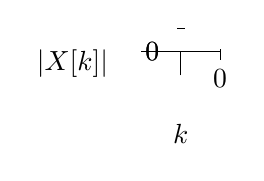
\begin{tikzpicture}[x=.5cm, y=0.3cm]

%axis
\draw (-2,0) -- coordinate (x axis mid)(0,0);
\draw (-1,-1) -- coordinate (y axis mid)(-1,0);

%ticks
\foreach \x in {0,...,0}
\draw (\x,1pt) -- (\x,-3pt)
node[anchor=north] {\x};

%ticks
\foreach \y in {0, 0}
\draw (-0.9,\y) -- (-1.1,\y)
node[left=0.1cm] {\y};

%ticks
\foreach \y in {1,...,0}
\draw (-0.9,\y) -- (-1.1,\y);

%label
\node[below=0.8cm] at (x axis mid) {$k$};
\node[left=0.8cm]   at (y axis mid) {$\left| X[k] \right|$};

\end{tikzpicture}
\end{document}
